
%(BEGIN_QUESTION)
% Copyright 2013, Tony R. Kuphaldt, released under the Creative Commons Attribution License (v 1.0)
% This means you may do almost anything with this work of mine, so long as you give me proper credit

Suppose you are asked to configure the instruments in this level control loop to sense and display process level over a range of 10 to 40 inches, with the loop controller actuating two split-ranged control valves in an exclusive sequence:

$$\includegraphics[width=15.5cm]{i02080x01.eps}$$

Write the proper range values inside the boxes near each instrument, showing the proper configuration for each instrument needed to achieve the desired result.

\vskip 20pt \vbox{\hrule \hbox{\strut \vrule{} {\bf Suggestions for Socratic discussion} \vrule} \hrule}

\begin{itemize}
\item{} Suppose the controller displayed a level of 28 when the actual process level was 22 inches.  First, identify {\it two} possible locations in this loop for a calibration error that would account for this discrepancy.  Then, assuming only one fault, explain how you could positively determine the location of this calibration error with a single diagnostic test.
\item{} Suppose valve LV-A was 58\% open and LV-B was 0\% open when the controller output displayed 25\%.  First, identify {\it three} possible locations in this loop for a calibration error that would account for this discrepancy.  Then, assuming only one fault, explain how you could positively determine the location of this calibration error with no more than two diagnostic tests.
\end{itemize}

\underbar{file i02080}
%(END_QUESTION)





%(BEGIN_ANSWER)

$$\includegraphics[width=15.5cm]{i02080x02.eps}$$

%(END_ANSWER)





%(BEGIN_NOTES)

A PV measurement error could lie within the transmitter, or within the controller's analog input.  A single current measurement of the transmitter's signal will tell you where the calibration error resides.

\vskip 10pt

A valve positioning error affecting LV-A (LV-B could also be affected, but we do not know because it's supposed to be saturated at 0\% at this controller output value) could lie within LV-A's positioner, the I/P transducer, or within the controller's analog output.  A single current measurement of the controller's output signal will tell you if a calibration error resides in the controller.  A pressure measurement at the I/P output will tell you if a calibration error resides in the valve positioner.  Comparing these two measurements will tell you if a calibration error resides in the I/P.

%INDEX% Basics, transmitter: input and output ranges
%INDEX% Final Control Elements, valve: split ranging

%(END_NOTES)

